\xchapter{Related Work and Present Solutions}{}\label{chapter:related} 
\textcolor{red}{Escrever introdução}
\section{Related Work in document variability}{}


The main contribution of our research is a variability based approach to support customised communication of the emergencies and its consequences targeted to proper audiences. Because of this, we explore the literature in order to identify related work in document variability.

There are proposals in the literature focusing exploring variability management techniques to build customised information for specific stakeholders. The information is usually represented by documents, as proposed by  \cite{penades2010}, which describes a process model for mass customisation of documents called Document Product Lines (DPL). Relying on SPL principles \citep{clements2002}, this work uses feature models \citep{Kang1990} to manage common and variable aspects of software development documents. The process model is realised by  DPLfw \citep{gomez2012dplfw}, a high-level design solution to support specialists on describing the variability of documents accordingly. DPLfw has been applied in several business domains to generate different DPLs (e.g. emergency plans \citep{gomez2012dplfw}, software manuals \citep{penades2012}, e-government \citep{penades2014},  customised recipes \citep{canos2013} and e-learning objects \citep{labib2015}). The DPLfw presents a complex process to specify and customise the document, this process is appropriated to large documents which demand large time intervals for your composition, not being proper to emergency public communication for not presenting such characteristics.

Karol et al. \citep{Karol2010} propose a tool for generating families of documents called Document Feature Mapper. This work also uses feature models to manage variability on families of documents. Each feature represents a fragment of the document (e.g. paragraphs, images) which varies as required. Despite the authors mapping the variability in several aspects, do not be considered the generating of documents in different formats, this is necessary for the dissemination of public communication using multiple communication channels. 

\cite{Rabiser2010} present an approach for automatic generation of product lines documents. They use the DOPLER \citep{rabiser2009} tool suite for modelling software artefacts and their respective variability and applies a Document Type Definition (DTD) called DOCBOOK \citep{walsh1999} for documents generation. Since this approach addresses the generation of product line documents, it cannot be applied to any other domain, such as public communication of emergencies.

%Limitações presentes em todos os papers
Public communication of emergencies requires the ability to build customised documents according to the audience in a quick way and deliver it considering all available communication infrastructures. The above mentioned proposals do not present solutions to cope with variability in communication network infrastructures. Furthermore, their tool support is limited, offering only plugins for the Eclipse\footnote{Eclipse - http://www.eclipse.org} Integrated Development Environment (IDE). Such an environment supports software development activities, it is not targeted to any other kinds of audience.

%como nosso trabalho atende às limitações dos outros artigos
Our proposal is designed to assist the public communication team. To do this, we design an assisted message edition of public communication models that vary, automatically, according to the emergency state. This allows the generation of specific messages according to the interest of each target groups from a unique public communication model.

\Section{Present solutions for public communication of emergencies} \label{chapter:PresentSolution}

There are several solutions for communication with civilians in case of an emergency. Some of them are used for public communication, while others are used for the guidance of the people involved in the emergency. 

In this section, we present some public communication solutions and highlight their main features. 
  

\subsection*{Twitter Alerts}

The social network Twitter\footnote{https://twitter.com} has developed a tool called “Twitter Alerts” \cite{twitteralerts}, whose goal is to provide authorities with a new way of disseminating information about an emergency. The Twitter alerts are disseminated with a specific visual identity via SMS and to twitter users. Figure \ref{fig:twitter} shows an example of Twitter Alerts. The image on the left shows the Twitter Alerts received by SMS and the image on the right shows a Twitter Alert received at the Twitter Mobile Application. To receive such notifications one must subscribe to the Twitter Alerts service.

\begin{figure}[]
\begin{center}
  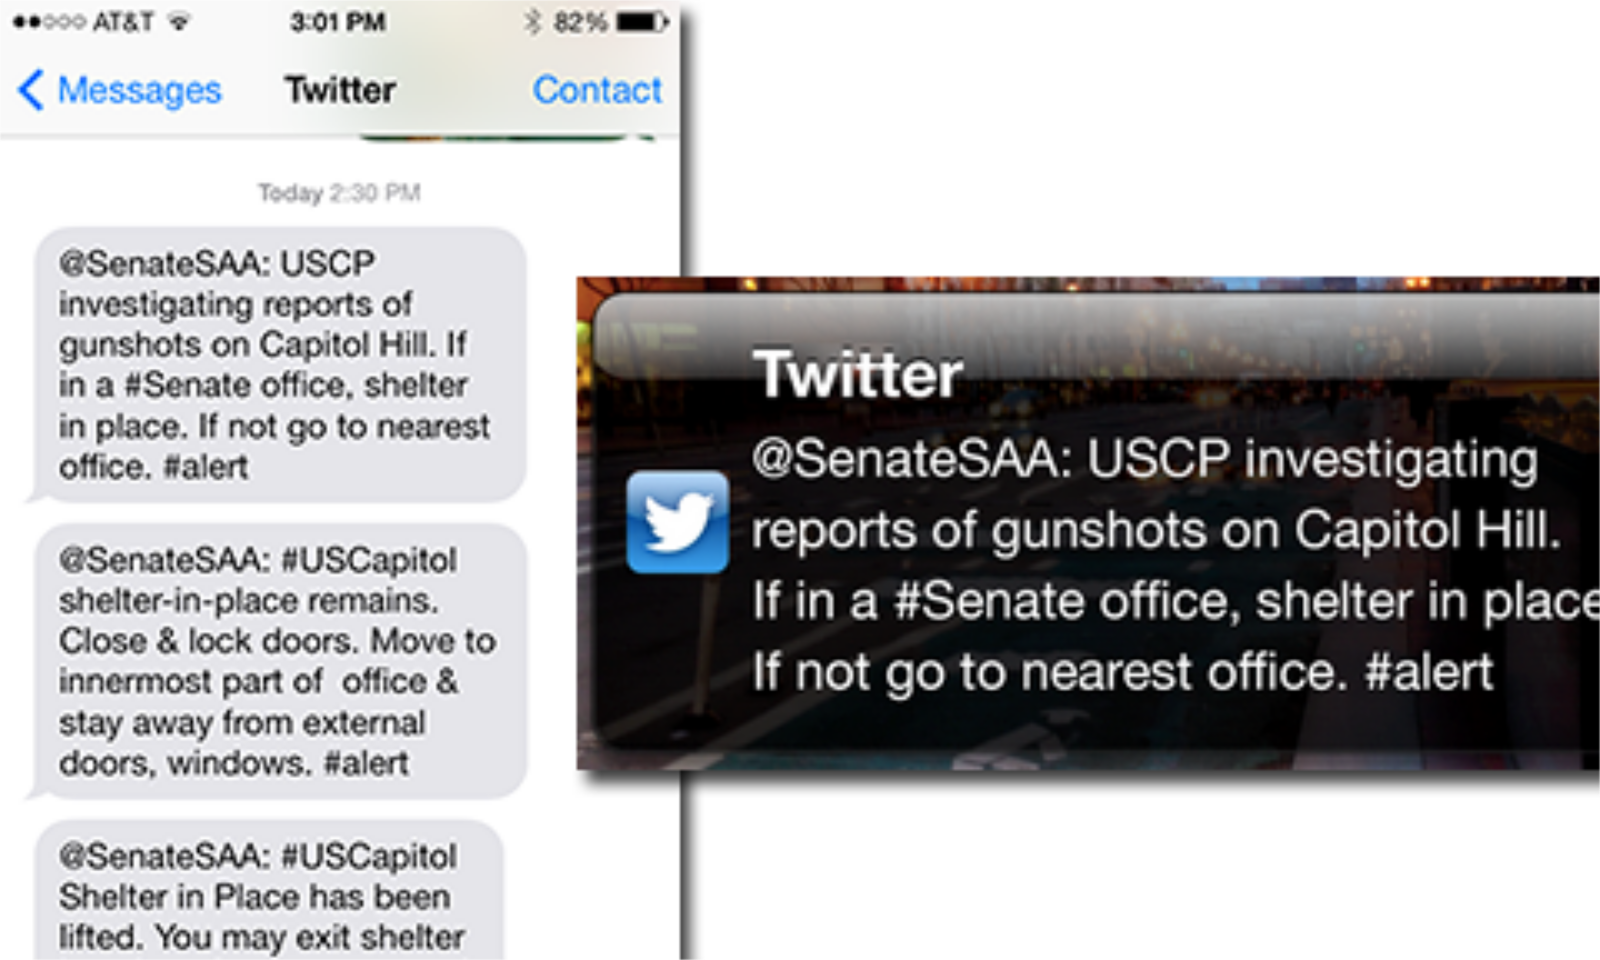
\includegraphics[width=0.7\linewidth, keepaspectratio]{twitterAlerts}
\caption{Example of Twitter Alerts messages. On the left an example of Twitter Alert Message notified by SMS and on the right by Twitter Mobile Application.}
\label{fig:twitter}
\end{center}
\end{figure}

\subsection*{Google Public Alerts}

Google Public Alerts is described as “a platform for disseminating relevant emergency alerts to users when and where they are searching for” \cite{googleAlerts}. The users are warned in two ways: a) by automatic emergency notifications sent through the mobile app Google Now (Android and IOS) and b) by customised search results when the user is looking for the situation of a specific emergency in the Google search engine. Figure \ref{fig:googleAlert} shows an example of search result (left side) and the emergency notification in Google Now (right side).

\begin{figure}[]
\begin{center}
  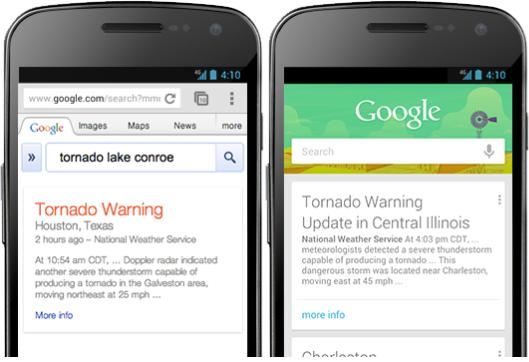
\includegraphics[width=0.7\linewidth, keepaspectratio]{googleAlerts}
\caption{Interface of Google Alert}
\label{fig:googleAlert}
\end{center}
\end{figure}

%\subsection*{Cell Broadcast Emergency Alerts}

%Cell Broadcast Emergency Alerts is a communication channel where messages can be issued to people in a specific area [13]. To receive emergency messages, the user’s mobile device must support the technology and the mobile telecommunication company must make the cell broadcast communication infrastructure available. Unlike SMS communication, solutions based on cell broadcast are free of network congestion, since such messages use an exclusive channel. Figure 3 shows an example of message received using this technology.

%\begin{figure}[htbp]
%\begin{center}
%  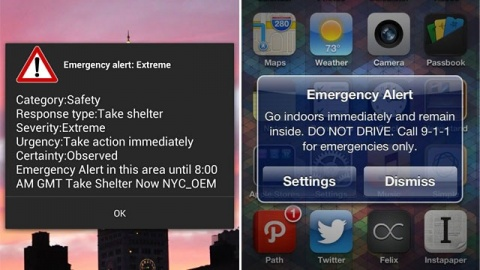
\includegraphics[height=5cm]{CellBroadcast}
%\caption{Examples of Cell Broadcast Emergency Alerts}
%\label{default-regular1}
%\end{center}
%\end{figure}

%There are governmental applications being developed for emergency communication using cell broadcast. For example, in the United States, the Commercial Mobile Alert System (CMAS) and the Wireless Emergency Alerts (WEA) [14], and, in the Netherlands, the NL-Alert [15]).

\subsection*{Israel National Message}

Developed by the Israeli government, the Israel National Message solution aims to “strengthen the spirit of the population and minimise subsequent damage in periods of war, national disasters and environmental emergency events by establishing a nationwide warning system that disseminates selective alerts and guidance messages to the population in real time, based on immediate control of all available and relevant channels in Israel” \cite{nationalMessage}. Figure \ref{fig:israelNM} presents the interface of the desktop solution.

\begin{figure}[]
\begin{center}
  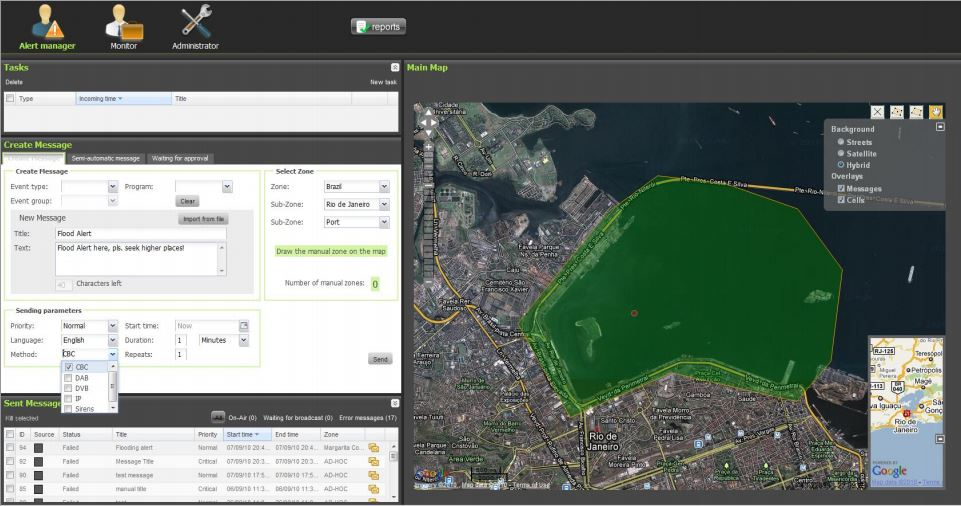
\includegraphics[width=0.85\linewidth, keepaspectratio]{israelNM}
\caption{Israel National Message (Personal Message Module)}
\label{fig:israelNM}
\end{center}
\end{figure}

This solution has a specific module for public communication called Personal Message, which allows the notification of an emergency occurrence to the population inside a specific area. This message can be sent by: cell broadcast, cell voice message, pager, TV, Radio, e-mail, website, Earthquake and Tsunami Warning service (ETWS) and sirens.

\subsection*{Alerts4All}
Alerts4All is a project developed in cooperation by 12 European partners. Its goal is to create “a complete communication framework for public alert” \cite{parraga2013complete}. This solution supports authorities during the preparation of emergency messages (Figure \ref{fig:allert4All}) and provides a specific communication protocol to transmit such messages. Therefore, it is necessary that TV, cell voice message, SMS, radio, GPS Navigator and sirens manufacturers implement the communication protocol created in the project. Figure \ref{fig:alert4allAlert} presents a practical example of alert message on TV.

\begin{figure}[]
\begin{center}
  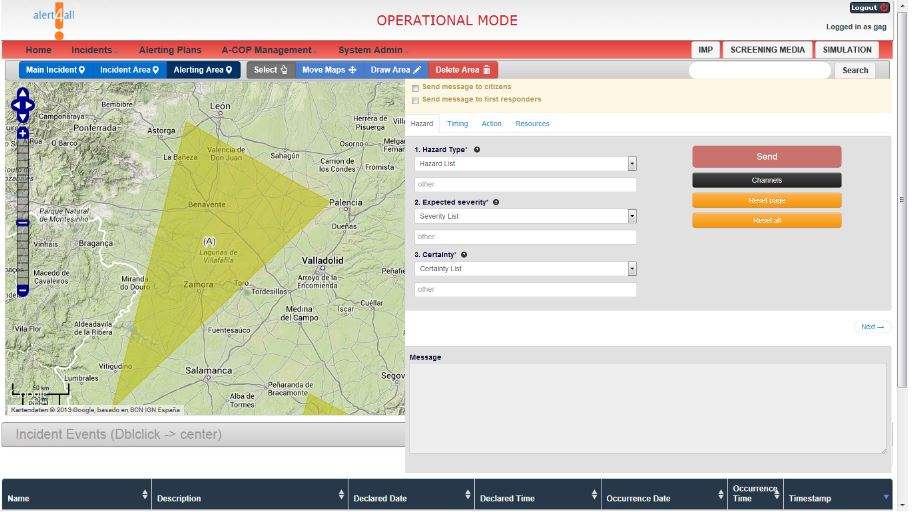
\includegraphics[width=0.8\linewidth, keepaspectratio]{alert4all}
\caption{Graphical user interface (GUI) of ALERT4ALL}
\label{fig:allert4All}
\end{center}
\end{figure}

\begin{figure}[]
\begin{center}
  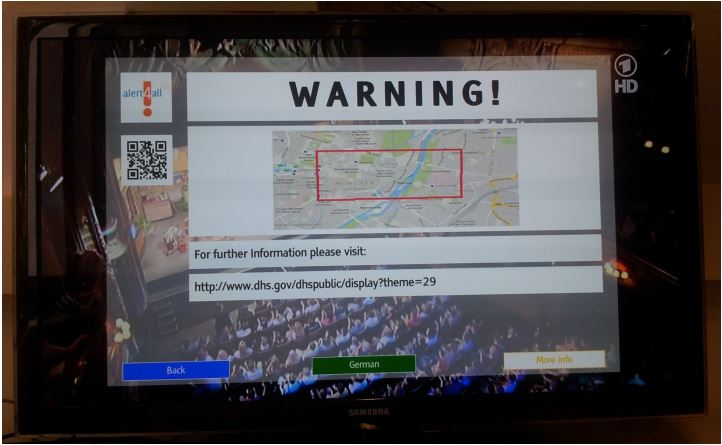
\includegraphics[width=0.8\linewidth, keepaspectratio]{alert4allAlert}
\caption{ALERT4ALL Alert Message on TV}
\label{fig:alert4allAlert}
\end{center}
\end{figure}

\subsection*{Code Red}

\begin{figure}[]
\begin{center}
  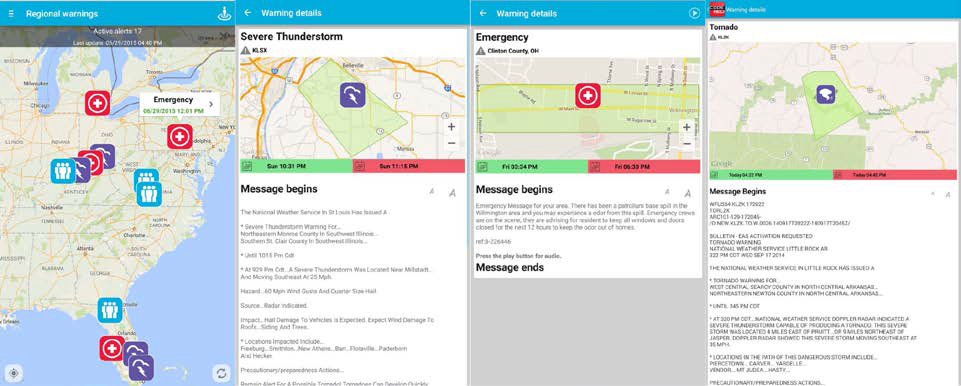
\includegraphics[width=0.8\linewidth, keepaspectratio]{codeRed}
\caption{Application screens of CodeRED Mobile Alert}
\label{fig:codRed}
\end{center}
\end{figure}

CodeRED (Figure \ref{fig:codRed}) is a solution developed by a company named Emergency Communication Network (ECN)\footnote{https://ecnetwork.com/} to support companies and authorities in reaching their audience during crisis and emergency situations. The audience can be notified by phone call, text message, e-mail, social media and CodeRED Mobile Alert application. Furthermore, the CodeRED is integrated with the Federal Emergency Management Agency (FEMA)\footnote{https://www.fema.gov/} of United States (U.S) and therefore allows sending alerts by WEA (Wireless Emergency Alerts)\footnote{https://www.fcc.gov/consumers/guides/wireless-emergency-alerts-wea}.

The emergency communicators can send messages using the web interface or by the mobile application called ACN Launcher (Figure \ref{fig:ecnLauncher}). CodeRED is in use by companies and public organisations in the United States and Canada.

\begin{figure}[]
\begin{center}
  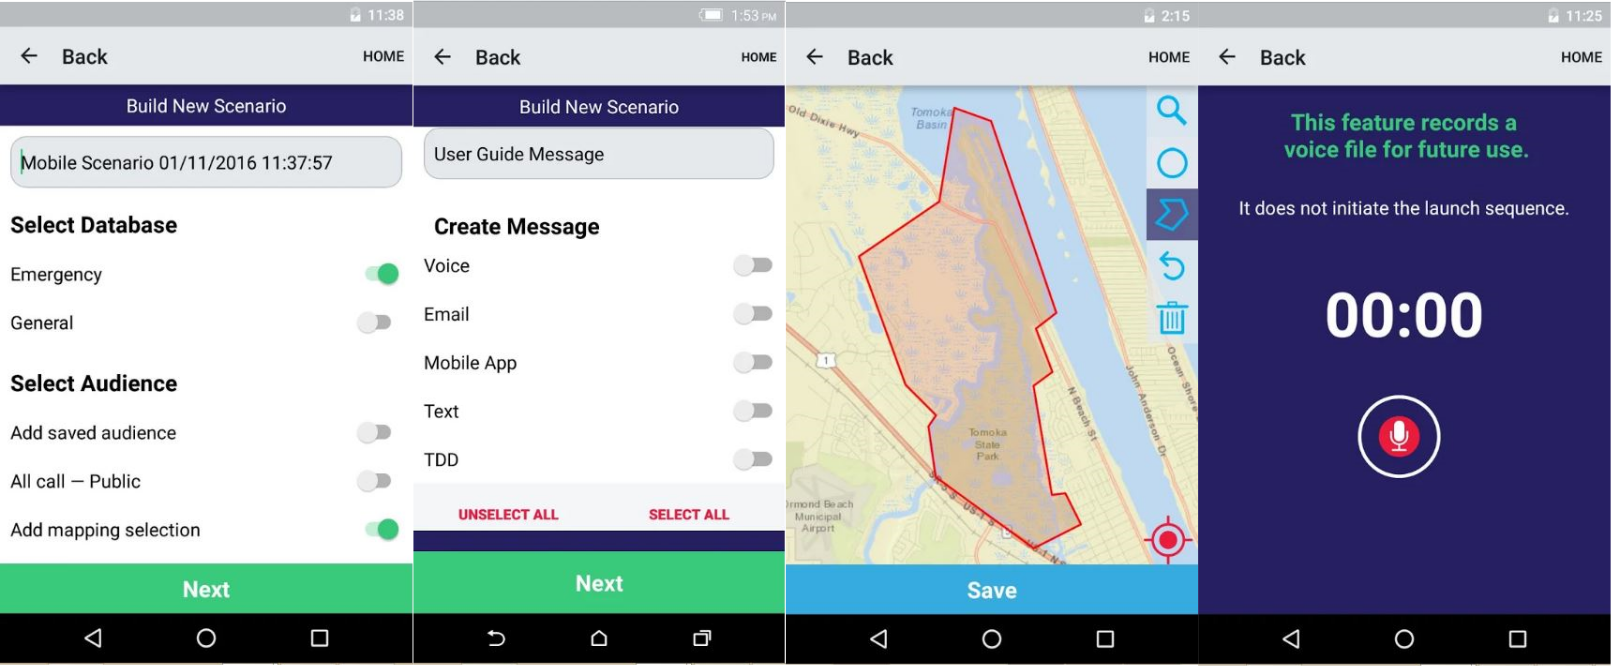
\includegraphics[width=0.6\linewidth, keepaspectratio]{ecnLauncher}
\caption{Application screens of ACN Launcher}
\label{fig:ecnLauncher}
\end{center}
\end{figure}

\subsection*{Crisis Communication Center}

\begin{figure}[]
\begin{center}
  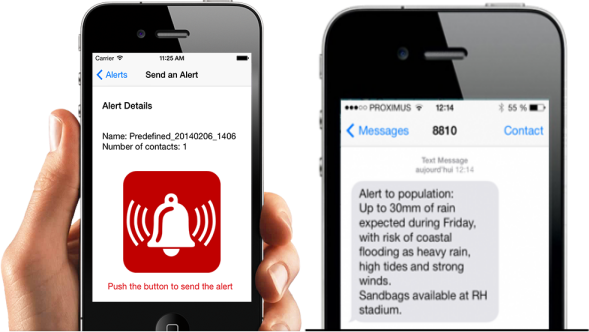
\includegraphics[width=0.6\linewidth, keepaspectratio]{crisisCC}
\caption{Application screens of Crisis Communication Center}
\label{fig:crisisCC}
\end{center}
\end{figure}

Crisis Communication Center is a crisis communication tool developed by the Belgian company “The Ring Ring”\footnote{http://www.ringring.be/}. The tool is a web-based solution that provides as main features the possibility of sending alerts by SMS, voice and e-mail. In addition, the tool allows the definition of message templates and includes the possibility of sending messages using a mobile application (Figure \ref{fig:crisisCC}).



\subsection{Limitations of the Existing Solutions}





Table \ref{comparisonTab} presents a comparison among the features present in the existing solutions. The following aspects were considered: assistance on the creation of messages (semi-automatic messages), sending of messages to specific areas (georeferenced) and the possibility of customisation of messages to specific groups of stakeholders. 

The aforementioned solutions are effective in disseminating reliable information about the emergency. However, the process of public communication of crisis/emergencies cannot be summarised to the sending of communications. Keeping the flow of reliable information to the communicator and helping him in the task of creating messages is crucial to ensure that this activity will be performed in an effective and efficient manner. 

In addition, the aforementioned solutions are not designed to create different messages for different target groups (e.g., press, public authorities or civilians). This is considered communication failures. This statement is based on the premise that “in a crisis, people don’t want to ‘just pick one’ of many messages, they want the best one or the right one to follow” \cite{reynolds2007crisis}.


% Please add the following required packages to your document preamble:
% \usepackage{booktabs}
% \usepackage[table,xcdraw]{xcolor}
% If you use beamer only pass "xcolor=table" option, i.e. \documentclass[xcolor=table]{beamer}
% Please add the following required packages to your document preamble:
% \usepackage{booktabs}
% \usepackage[table,xcdraw]{xcolor}
% If you use beamer only pass "xcolor=table" option, i.e. \documentclass[xcolor=table]{beamer}
\begin{table}[]
\centering
\caption{Comparison of Existing Solutions}
\label{comparisonTab}
\begin{tabular}{@{}llccc@{}}
\rowcolor[HTML]{9BBB59} 
{\color[HTML]{FFFFFF} Solution}                                                                                                    & {\color[HTML]{FFFFFF} Communication Technology}                                                                                                              & {\color[HTML]{FFFFFF} \begin{tabular}[c]{@{}c@{}}Message\\ Templates\end{tabular}}                       & {\color[HTML]{FFFFFF} \begin{tabular}[c]{@{}c@{}}Group-targeted\\ Customization\end{tabular}} & {\color[HTML]{FFFFFF} \begin{tabular}[c]{@{}c@{}}Location \\ based\\ Messages\end{tabular}} \\ \midrule
\rowcolor[HTML]{EAF1DD} 
\multicolumn{1}{|l|}{\cellcolor[HTML]{EAF1DD}\textbf{Twitter Alerts}}                                                              & \multicolumn{1}{l|}{\cellcolor[HTML]{EAF1DD}\begin{tabular}[c]{@{}l@{}}Mobile Application, Website \\ and SMS\end{tabular}}                                  & \multicolumn{1}{c|}{\cellcolor[HTML]{EAF1DD}No}                                                          & \multicolumn{1}{c|}{\cellcolor[HTML]{EAF1DD}No}                                               & \multicolumn{1}{c|}{\cellcolor[HTML]{EAF1DD}No}                                             \\ \midrule
\rowcolor[HTML]{FFFFFF} 
\multicolumn{1}{|l|}{\cellcolor[HTML]{FFFFFF}\textbf{\begin{tabular}[c]{@{}l@{}}Google Public\\ Alerts\end{tabular}}}              & \multicolumn{1}{l|}{\cellcolor[HTML]{FFFFFF}\begin{tabular}[c]{@{}l@{}}Mobile Application\\ and Website\end{tabular}}                                        & \multicolumn{1}{c|}{\cellcolor[HTML]{FFFFFF}No}                                                          & \multicolumn{1}{c|}{\cellcolor[HTML]{FFFFFF}No}                                               & \multicolumn{1}{c|}{\cellcolor[HTML]{FFFFFF}Yes}                                            \\ \midrule
\rowcolor[HTML]{EAF1DD} 
\multicolumn{1}{|l|}{\cellcolor[HTML]{EAF1DD}\textbf{\begin{tabular}[c]{@{}l@{}}Cell Broadcast\\ Emergency\\ Alerts\end{tabular}}} & \multicolumn{1}{l|}{\cellcolor[HTML]{EAF1DD}Cell Broadcast}                                                                                                  & \multicolumn{1}{c|}{\cellcolor[HTML]{EAF1DD}No}                                                          & \multicolumn{1}{c|}{\cellcolor[HTML]{EAF1DD}No}                                               & \multicolumn{1}{c|}{\cellcolor[HTML]{EAF1DD}Yes}                                            \\ \midrule
\multicolumn{1}{|l|}{\textbf{\begin{tabular}[c]{@{}l@{}}National\\ Message\end{tabular}}}                                          & \multicolumn{1}{l|}{\begin{tabular}[c]{@{}l@{}}Website, Cell Broadcast,\\ Cell, Voice Message, \\ Pager, TV, Radio, E-mail,\\ ETWS and Sirens.\end{tabular}} & \multicolumn{1}{c|}{\begin{tabular}[c]{@{}c@{}}Yes\\ (Static text)\end{tabular}}                         & \multicolumn{1}{c|}{No}                                                                       & \multicolumn{1}{c|}{Yes}                                                                    \\ \midrule
\rowcolor[HTML]{EAF1DD} 
\multicolumn{1}{|l|}{\cellcolor[HTML]{EAF1DD}\textbf{Alerts4All}}                                                                  & \multicolumn{1}{l|}{\cellcolor[HTML]{EAF1DD}\begin{tabular}[c]{@{}l@{}}Cell Voice Message, SMS,\\ TV, Radio, GPS Navigator\\ and Sirens.\end{tabular}}       & \multicolumn{1}{c|}{\cellcolor[HTML]{EAF1DD}\begin{tabular}[c]{@{}c@{}}Yes\\ (Static text)\end{tabular}} & \multicolumn{1}{c|}{\cellcolor[HTML]{EAF1DD}No}                                               & \multicolumn{1}{c|}{\cellcolor[HTML]{EAF1DD}Yes}                                            \\ \midrule
\multicolumn{1}{|l|}{\textbf{Code Red}}                                                                                            & \multicolumn{1}{l|}{\begin{tabular}[c]{@{}l@{}}Mobile Application, SMS,\\ Cell Voice Message, E-mail,\\ and Social Networks\end{tabular}}                    & \multicolumn{1}{c|}{\begin{tabular}[c]{@{}c@{}}Yes\\ (Static text)\end{tabular}}                         & \multicolumn{1}{c|}{No}                                                                       & \multicolumn{1}{c|}{Yes}                                                                    \\ \midrule
\rowcolor[HTML]{EAF1DD} 
\multicolumn{1}{|l|}{\cellcolor[HTML]{EAF1DD}\textbf{\begin{tabular}[c]{@{}l@{}}Crisis\\ Communication\\ Center\end{tabular}}}     & \multicolumn{1}{l|}{\cellcolor[HTML]{EAF1DD}\begin{tabular}[c]{@{}l@{}}Mobile Application, SMS,\\ Cell Voice Message\\ and E-mail\end{tabular}}              & \multicolumn{1}{c|}{\cellcolor[HTML]{EAF1DD}\begin{tabular}[c]{@{}c@{}}Yes\\ (Static text)\end{tabular}} & \multicolumn{1}{c|}{\cellcolor[HTML]{EAF1DD}No}                                               & \multicolumn{1}{c|}{\cellcolor[HTML]{EAF1DD}Yes}                                            \\ \bottomrule
\end{tabular}
\end{table}

%Some communication technologies were not implemented in our solution. This decision was justified due to the fact that some communication technologies are restrict to governmental organizations (cell broadcast, TV and Sirens) or implies in additional costs (cell voice message). However, our solution was designed to allow the integration with others communication technologies and their respective message formats. We analysed the possible variability points in our solution to ensure its configuration to other scenarios, such other communication technologies.